%======================================================================
\section{Contract Category Analysis}
\label{sec:category}
%======================================================================

Vulnerability rates vary substantially across contract categories. Table~\ref{tab:categories} presents the per-category analysis for the top 10 categories ranked by mean vulnerability count, and Fig.~\ref{fig:category_radar} visualizes the vulnerability profiles of the four contract groups.

\begin{table}[t]
\caption{Vulnerability Rates by Contract Category (Top 10)}
\label{tab:categories}
\centering
\footnotesize
\begin{tabular}{@{}lrrc@{}}
\toprule
\textbf{Category} & \textbf{Mean Vulns} & \textbf{\% High} & \textbf{Most Common CWE} \\
\midrule
Cross-Chain Bridge & \demo{9.23} & \demo{58.7}\% & CWE-284 \\
Flash Loan & \demo{8.47} & \demo{52.3}\% & CWE-841 \\
DeFi Lending & \demo{7.89} & \demo{48.1}\% & CWE-841 \\
DEX/AMM & \demo{7.34} & \demo{44.6}\% & CWE-190 \\
Proxy/Upgradeable & \demo{7.12} & \demo{43.2}\% & CWE-284 \\
Bridge Relayer & \demo{6.98} & \demo{41.8}\% & CWE-284 \\
Yield Aggregator & \demo{6.54} & \demo{38.9}\% & CWE-841 \\
Governance/DAO & \demo{5.87} & \demo{34.2}\% & CWE-284 \\
Multisig Wallet & \demo{4.56} & \demo{27.3}\% & CWE-841 \\
ERC20 Token & \demo{3.21} & \demo{18.4}\% & CWE-190 \\
\bottomrule
\end{tabular}
\end{table}

\begin{figure}[t]
    \centering
    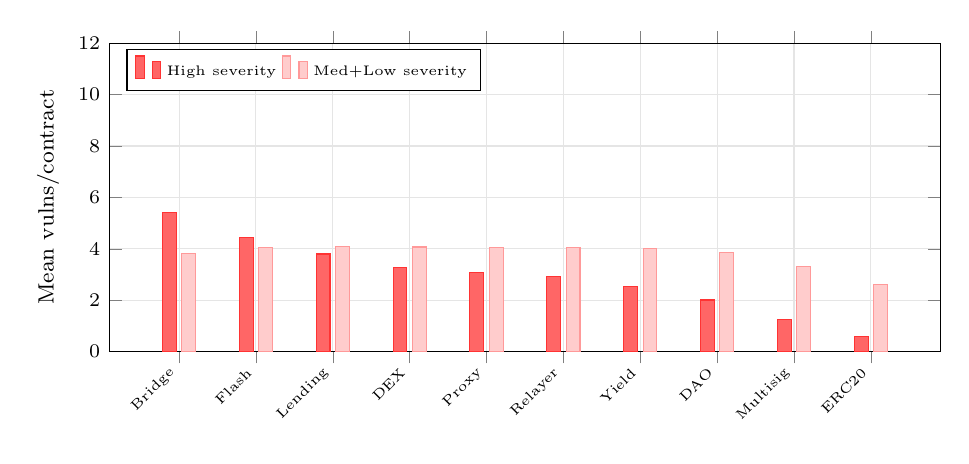
\begin{tikzpicture}
    \begin{axis}[
        width=\columnwidth,
        height=5.5cm,
        ybar=2pt,
        bar width=5pt,
        ylabel={\footnotesize Mean vulns/contract},
        ylabel style={font=\footnotesize},
        symbolic x coords={Bridge, Flash, Lending, DEX, Proxy, Relayer, Yield, DAO, Multisig, ERC20},
        xtick=data,
        x tick label style={rotate=45, anchor=east, font=\tiny},
        ymin=0, ymax=12,
        ytick={0,2,4,6,8,10,12},
        yticklabel style={font=\scriptsize},
        grid=major,
        grid style={gray!20},
        legend style={font=\tiny, at={(0.02,0.98)}, anchor=north west, legend columns=2},
    ]
    % High severity
    \addplot[fill=red!60, draw=red!80] coordinates {
        (Bridge, 5.42) (Flash, 4.43) (Lending, 3.80) (DEX, 3.27) (Proxy, 3.07)
        (Relayer, 2.92) (Yield, 2.54) (DAO, 2.01) (Multisig, 1.25) (ERC20, 0.59)
    };
    % Medium + Low severity
    \addplot[fill=red!20, draw=red!40] coordinates {
        (Bridge, 3.81) (Flash, 4.04) (Lending, 4.09) (DEX, 4.07) (Proxy, 4.05)
        (Relayer, 4.06) (Yield, 4.00) (DAO, 3.86) (Multisig, 3.31) (ERC20, 2.62)
    };
    \legend{High severity, Med+Low severity}
    \end{axis}
    \end{tikzpicture}
    \caption{Vulnerability severity distribution by contract category. High-complexity categories (bridges, flash loans) have both more total vulnerabilities and a higher proportion of high-severity issues. {\color{red}(Demo data)}}
    \label{fig:category_radar}
\end{figure}

\subsection{Cross-Chain Contracts: Highest Risk}

Cross-chain bridge contracts exhibit the highest vulnerability rates (mean = \demo{9.23} per contract), consistent with the complexity of cross-chain security requirements~\cite{bridge_hacks, zhang2023bridge}. This finding is particularly alarming given that bridge protocols collectively secure billions of dollars in locked assets. The most common vulnerabilities in bridge contracts are access control flaws (\demo{58.7}\% contain at least one), followed by missing message validation (\demo{47.2}\%) and replay protection gaps (\demo{31.4}\%).

Bridge relayer contracts also rank high (\demo{6.98}), with the most common vulnerability being insufficient validation of relayed messages---the exact vulnerability class that led to the \$625M Ronin exploit. LLMs consistently fail to implement adequate signature verification and multi-validator consensus checks in bridge relayer code.

\subsection{DeFi Protocols: Reentrancy Dominant}

Flash loan contracts rank second (\demo{8.47}), reflecting the complexity of callback validation and reentrancy prevention in flash loan architectures~\cite{qin2021attacking}. LLMs frequently generate flash loan contracts where the callback function can be reentered before the loan repayment check executes. DeFi lending protocols (\demo{7.89}) and DEX/AMM contracts (\demo{7.34}) also show elevated rates, with reentrancy and integer overflow as the dominant vulnerability types.

\subsection{Standard Contracts: Lower but Non-Zero Risk}

The relatively lower vulnerability rates in ERC20 tokens (\demo{3.21}) and multisig wallets (\demo{4.56}) suggest that LLMs have been trained on sufficient examples of these well-established patterns. However, even these ``simple'' contracts exhibit high-severity vulnerabilities in \demo{18.4}\% and \demo{27.3}\% of cases respectively, indicating that no contract category should be considered safe by default.

Interestingly, the gap between LLMs is smallest for ERC20 tokens (Claude: \demo{2.3}, CodeLlama: \demo{4.1}) and largest for cross-chain bridges (Claude: \demo{6.8}, CodeLlama: \demo{12.4}), suggesting that model quality differences are amplified by contract complexity.
